\documentclass{beamer}
\usepackage[utf8]{inputenc}

\usepackage{graphicx}

\usetheme{Boadilla}

\title[SybilGuard]{SybilGuard:\\ Defending Against Sybil Attacks via Social Networks}
\author[Dagand, Jezequel]{H. {\sc Yu} \and M. {\sc Kaminsky} \and P. {\sc Gibbons} \and A. {\sc Flaxman}\\
                          Pierre-Evariste {\sc Dagand} \and Loïg {\sc Jezequel}}
\date{January $14^{\mbox{th}}$, 2009}
\institute[PAP]{Pair-à-Pair}

\begin{document}

%%%%%%%%%%%%%%%%%%%%%%%%%%%%%%%%%%%%%%%%%%%%%%%%%%%%%%%%%%%%%%%%

\begin{frame}
\maketitle
\end{frame}

%%%%%%%%%%%%%%%%%%%%%%%%%%%%%%%%%%%%%%%%%%%%%%%%%%%%%%%%%%%%%%%%

\begin{frame}

  \frametitle{Introduction}

  \begin{block}{Sybil Attacks}
    \begin{description}
      \item[Definition:] A malicious user endorses multiple identities  %% Improve this definition ?
      \item[Impact:] Most distributed systems expect a majority of honest users\\
	             Eg.: 2/3 for Byzantine Consensus
    \end{description}
  \end{block}

  \begin{block}{Theoretical Result}
    \begin{description}
      \item[(Douceur02):] ``Thou cannot pass out Sybil nodes in a distributed manner'' %% Find the exact quote...
      \item[Consequence:] Rely on a Central Authority? 
    \end{description}
  \end{block}

\end{frame}

%%%%%%%%%%%%%%%%%%%%%%%%%%%%%%%%%%%%%%%%%%%%%%%%%%%%%%%%%%%%%%%%

\begin{frame}

  \frametitle{SybilGuard}

  \begin{block}{Offering Weaker Guarantees}

    \begin{columns}

      \begin{column}{7cm}
	\begin{itemize}
	\item Bound the number of Sybil nodes
	\item Bound the number of Sybil groups
	\item Accept honest nodes
	\end{itemize}
      \end{column}

      \begin{column}{4cm}
	\vfill
	{\it With High-Probability!}
	\vfill
      \end{column}

    \end{columns}

  \end{block}

  \begin{block}{Benefits}

    \begin{itemize}
      \item Fully decentralized
      \item Handle network dynamics
      \item Leverage Social Networks
    \end{itemize}

  \end{block}

\end{frame}

%%%%%%%%%%%%%%%%%%%%%%%%%%%%%%%%%%%%%%%%%%%%%%%%%%%%%%%%%%%%%%%%

\begin{frame}

  \frametitle{Social Network}
  
  \begin{figure}
    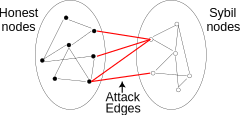
\includegraphics[width=7cm]{./pictures/social_network} \\
    \caption{Social Network}
  \end{figure}

  \begin{block}{Properties}

    \begin{itemize}
    \item Build upon strong trust relationships
    \item \emph{Attack edge}: small quotient cut
    \item Widely studied model
    \end{itemize}

  \end{block}

\end{frame}

%%%%%%%%%%%%%%%%%%%%%%%%%%%%%%%%%%%%%%%%%%%%%%%%%%%%%%%%%%%%%%%%

\begin{frame}

  \frametitle{Random Routes}

  \begin{figure}
    \begin{columns}
      \begin{column}{4.5cm}
	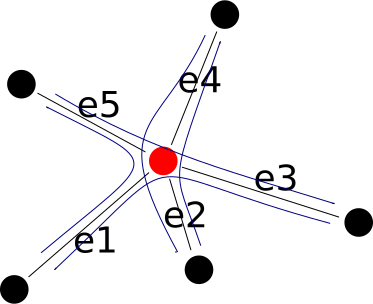
\includegraphics[width=4.5cm]{./pictures/random_route} 
      \end{column}
      \begin{column}{3cm}
	\begin{center}
	  \begin{tabular}{|c|c|c|c|c|}
	    \hline
	    $e_1$ & $e_2$ & $e_3$ & $e_4$ & $e_5$ \\
	    \hline
	    $e_5$ & $e_4$ & $e_1$ & $e_2$ & $e_3$ \\
	    \hline
	  \end{tabular}
	\end{center}
      \end{column}
    \end{columns}

    \caption{Random Routes}
  \end{figure}

  \begin{block}{Properties}
    \begin{description}
      \item[Convergence:] {\small \emph{Two random nodes entering an honest node along the same edge will always exit along the same edge}}
      \item[Back-traceability:] {\small \emph{The outgoing edge uniquely determines the incoming edge}}
    \end{description}
  \end{block}


\end{frame}


%%%%%%%%%%%%%%%%%%%%%%%%%%%%%%%%%%%%%%%%%%%%%%%%%%%%%%%%%%%%%%%%

\end{document}
